\documentclass[a4paper,11pt]{article}
\usepackage[latin1]{inputenc}
\usepackage[T1]{fontenc}
\usepackage[english]{babel}
% \usepackage{amsmath}
% \usepackage{amssymb,amsfonts,textcomp}
% \usepackage{color}
% \usepackage{array}
% \usepackage{supertabular}
% \usepackage{hhline}
\usepackage{hyperref}
\usepackage{cite}
% \usepackage{etoolbox}
\usepackage{acro}
\usepackage{graphicx}
\usepackage[nodayofweek]{datetime}

\acsetup{first-style=short}
\DeclareAcronym{rl}{
  short = RL ,
  long  = Reinforcement Learning,
  class = abbrev
}
\DeclareAcronym{ai}{
  short = AI ,
  long  = Artificial Intelligence,
  class = abbrev
}


\DeclareGraphicsRule{*}{mps}{*}{}

% Commands
\newcommand{\HRule}{\rule{\linewidth}{0.5mm}} % Defines a new command for the horizontal lines

\begin{document}

	\begin{titlepage}
		\begin{centering}
		 
		%	HEADING SECTIONS
		\textbf{\textit{\large{B.Tech Project Report}}}\\[0.5cm]
		
		\textsc{\textbf{\LARGE{Decision making using deep reinforcement learning}}}\\[1.5cm]

		\large{Submitted in partial fulfilment for the award of the Degree of Bachelor of Technology in Computer Science and Engineering}\\[1.5cm]

		\large{Submitted by}\\[0.5cm]

		\textbf{Jayadeep K M     (Roll No 13400030)}\\
		\textbf{Kevin Joseph     (Roll No 13400032)}\\
		\textbf{Mohammed Nisham K     (Roll No 13400038)}\\[1.5cm]
		
		{Under the guidance of}\\[0.25cm]
		\large{Mr. Vipin Vasu A V}\\[0.5cm]

		
\includegraphics[width=5cm]{images/logo.jpg} 

		Department of Computer Science and Engineering\\
		\textsc{College of Engineering, Trivandrum}\\
		\textsc{Kerala}\\
		\textsc{May 2017}\\
		\vfill % Fill the rest of the page with whitespace
		\end{centering}
	\end{titlepage}

	\begin{titlepage}
		\begin{centering}
			\textbf{\textit{\LARGE\textsc{{certificate}}}}\\[0.5cm]
			
\includegraphics[width=5cm]{images/logo.jpg}\\

		\end{centering}

		\large{This is to certify that the thesis entitled ``Decision making using deep reinforcement learning'' is a bonafide record of the major project done by \textbf{Jayadeep K M} (Roll No 13400030), \textbf{Kevin Joseph} (Roll No 13400032) and \textbf{Mohammed Nisham K} (Roll No 13400038) under my supervision and guidance, in partial fulfilment for the award of the Degree of Bachelor of Technology in Computer Science and Engineering from the University of Kerala for the year 2017.}\\[1.5cm]

		\begin{minipage}{0.4\textwidth}
		\begin{flushleft}
		\end{flushleft}
		\end{minipage}
		~
		\begin{minipage}{0.6\textwidth}
		\begin{centering} \large
		\large{Mr. Vipin Vasu A V}\\
		\small{(Guide)}\\
		\small{\textit{\textbf{Asst. Professor}}}\\
		\small{\textit{\textbf{Dept. of Computer Science and Engineering}}}\\[1.5cm]

		\large{Mrs. Liji}\\
		\small{\textit{\textbf{Professor and Head}}}\\
		\small{\textit{\textbf{Dept. of Computer Science and Engineering}}}\\
		\end{centering}
		\end{minipage}\\[1.0cm]

		\begin{flushleft}
		Place: Trivandrum\\
		Date:  11-05-2017\\
		\end{flushleft}
		\vfill % Fill the rest of the page with whitespace
	\end{titlepage}

	% TODO Ack before this
	\pagenumbering{roman}
	
	\begin{abstract}
		Creating a general purpose AI has been an area of research since the beginning of computers and programming. Reinforcement learning is a major step towards a general purpose AI. \\

		This project is aimed at creating a program that can learn to make decisions in an environment that is defined by a high-dimensional input, and has sparce and time delayed rewards for these actions. Such programs can be useful in problems where decsion must be made based on high dimensional sensory input such as camera feed. This project uses Q-learning algorithm to assign a quality value to each action in a state of the environment. \\

		Atari games are used to demonstrate this approach, by training the program to play breakout game for upto 50 epochs and observing performance improvement. The trained neural network was saved and tested at the end of every epoch. The performance parameters like average q-value, average reward, games per epoch were also saved. The performace parameters showed a clear rise in performace for breakout (50 epochs) and space invaders (8 epochs). \\

		The project has applications in the field of IOT, security, gaming, stock market analysis and traffic control systems. Any system that can be modelled as an environment with actions and rewards can be trained using this algorithm.

	\end{abstract}
	
	\newpage
	\tableofcontents
	\newpage
	\listoffigures
	\newpage
	\printacronyms[include-classes=abbrev,name=Abbreviations]
	\newpage

	\pagenumbering{arabic}
	\section{Introduction}
		\subsection{Motivation and Overview}
			Learning to control agents directly from high-dimensional sensory inputs like vision and speech is one of the long-standing challenges of Artificial Intelligence and Machine Learning. Most successful \ac{ai} applications have relied on hand-crafted features combined with linear value functions or policy representations. Clearly, the performance of such systems heavily relies on the quality of the feature representation.

			Recent advances in deep learning have made it possible to extract high-level features from raw sensory data, leading to breakthroughs in computer vision and speech recognition. These methods utilise a range of neural network architectures, including convolutional networks, multilayer perceptrons, restricted Boltzmann machines and recurrent neural networks, and have exploited both supervised and unsupervised learning.
	
			However the main advantage of Reinforcement Learning is that it does't need huge amounts of hand-labelled data and does not depend too much on the feature representation. It learns from a reward signal that maybe delayed, noisy and sparse. The delay between actions and the rewards, which maybe thousands of timesteps seems like a particularly hard problem in \ac{rl} when compared to direct association between action and reward in supervised learning. Another issue is that most problems consider all the data samples independent of each other, but in this case we need to consider the fact that the reward at the end of a session is not just the result of the last action but the result of the sequence of actions from the start of the session.

			This project is aimed at using a Convolution Neural Network along with the Q-learning algorithm to solve the above problems and make decisions based on video input from the Atari Learning Environment. Our goal is to create a single neural network agent that is able to successfully learn to play atleast 2 games with no change in agent algorithm. The network was not provided with any game-specific information or hand-designed visual features, and was not privy to then internal state of the emulator, it learned from nothing but the video input, the reward and terminal signals, and the set of possible actions just as a human player would.

		\subsection{Literature Survey}
			\paragraph{Deep Mind}

	\section{Materials and Methodology}
		\subsection{Algorithms}
			\subsubsection{Q-Learning}
			\subsubsection{Deep Q-Learning}
				\paragraph{Neural Networks}

		\subsection{Program Development}
			\subsubsection{System Description}
			\subsubsection{Class Diagram}
				\begin{figure}[!h]
					\begin{centering}
						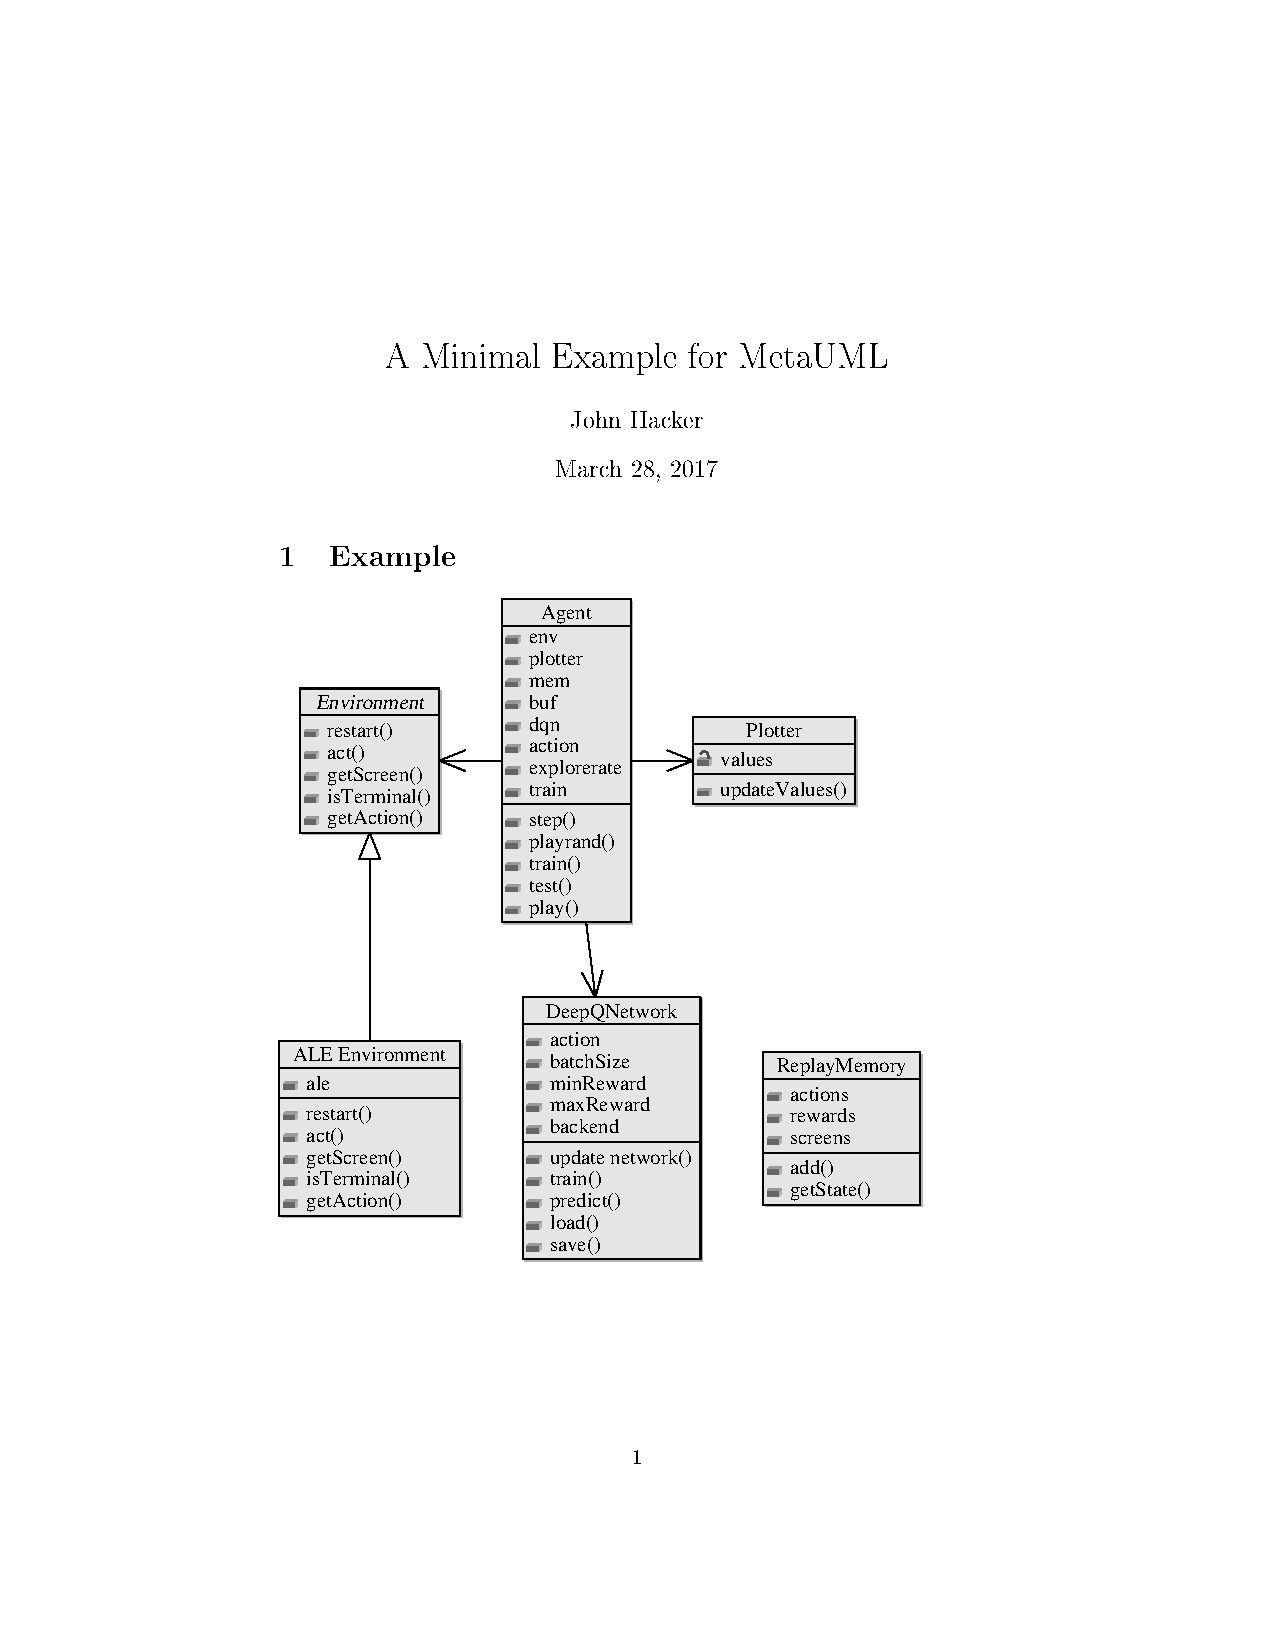
\includegraphics[width=15cm]{../uml/uml.1}
						\caption{UML Class Diagram.}
					\end{centering}
				\end{figure}
			\subsubsection{Code Overview}

	\section{Results and Discussions}
		\subsection{Description of observed strategies}
		\subsection{Screenshots}
		\subsection{Result Visualization}

	\section{Further Work}
		\subsection{Gamification of Problem}
			Solving real world problems can be achieved using Deep Reinforcement Learning. The following points are to be considered to convert a real world problem into a deep learning optimisation problem:
			\begin{itemize}
				\setlength\itemsep{0em}
				\item The problem is to be modelled as a game.
				\item The game should include an environment which has a finite set of actions.
				\item High dimensional input to the environment should be available as input and savable as a state.
				\item State of the system should change according to the actions performed on it.
				\item The environment should occasionally give off rewards in response to its current state or action performed.
			\end{itemize}

			If all of the criterions are met and a gamified version of the real world problem is made, then it can be quite easily given to a deep reinforcement learning system for optimisation and then later used in real life after training.

		\subsection{Traffic Light Control}
			\subsubsection{Problem}
				There is an intersection of two roads, and four traffic lights control the traffic in it, each controlling one road. The control of the traffic light should be given to an \ac{ai} for optimum traffic flow through the intersection. To design a system that can be used to train this \ac{ai}. 

			\subsubsection{Minimal Input}
				Traffic camera images at four different directions are taken as input to the system, mulitple images are taken to incorporate movement of the vehicles. Even though the system could work with the raw images, it would be impossible to train the system in the real world. So a simulation is required to train it. But in a simulation output images cannot be generated as complex as real video stream. 

				The solution is to simplify the input to the system, and to simulate the output in this simplified version. The approach taken is to convert the vehicles into white rectangles in a black canvas, and the intersection as a line. Thus white rectangles passing over the line will be taken for rewards and any intersection of rectangles will be interpreted as a crash. The rectangles are easier to simulate given the actions to be performed.

				To make the simulation closer to reality, delay between the signal turning green and the first car moving can be given. Contraction and elongation of traffic at stop and start can also be simulated.

				\begin{figure}[!h]
					\begin{centering}
						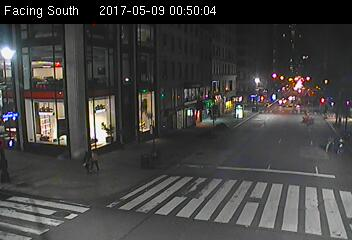
\includegraphics[width=15cm]{images/traffic1.png}
						\caption{Empty Intersection.}
					\end{centering}
				\end{figure}

				
				\begin{figure}[!h]
					\begin{centering}
						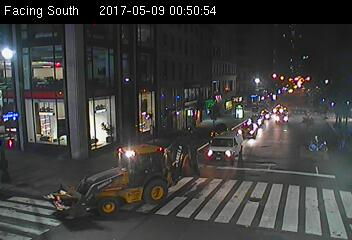
\includegraphics[width=15cm]{images/traffic2.png}
						\caption{Intersection with Vehicles.}
					\end{centering}
				\end{figure}

				
				\begin{figure}[!h]
					\begin{centering}
						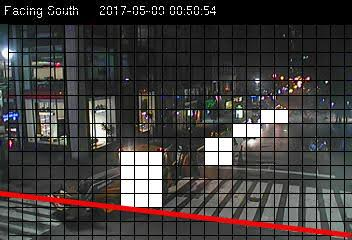
\includegraphics[width=15cm]{images/traffic3.png}
						\caption{Generation of Simplified Input.}
					\end{centering}
				\end{figure}

				
				\begin{figure}[!h]
					\begin{centering}
						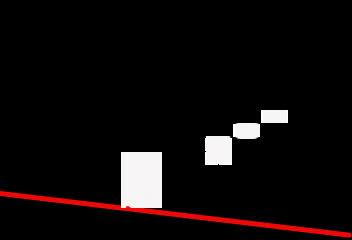
\includegraphics[width=15cm]{images/traffic4.png}
						\caption{Simplified Input.}
					\end{centering}
				\end{figure}



			\subsubsection{Action set}
				At any instant, any of the traffic lights can be any of the following:
				\begin{itemize}
					\setlength\itemsep{0em}
					\item Red
					\item Orange
					\item Green in the Right, Left, Straight direction or any combination of it.
				\end{itemize}

				Orange can be eliminated by making it mandatory for transitions between Green and Red. Green has seven states (not to be confused with state of the system found from the input) it can be in for all the combinations. Since only Green or Red can be active at a given time, the total no of states for a single traffic light is 8.

				The intersection consists of 4 traffic lights, operating independantly (No constraints to its operation) making the total no of actions the system can take to $8^4$ = 4096 actions.

				Thus at every state of the system, it can decide between 4096 actions to take.
			\subsubsection{Reward}
				The no of vehicles that pass through the intersection in a time interval or the throughput of the intersection can be taken as a rudimentary reward function.

				To avoid any traffic signals that might incur collisions, any collisions detected are penalised with a negative reward.

				This still presents the problem of starvation \emph{ie.} a low amount of vehicles could wait for green indefinitely. It can be solved by aging the throughput negatively, which makes the throughput reward smaller and finally negative the longer it waits.
			\subsubsection{Scalability}
				The system proposed could be implemented on a larger scale, like a town or city. But in the current form of neural networks, adding a single traffic light to an existing system makes retraining the entire system a requirement. As the number of intersections increase, the number of actions rise exponentially. Thus making their efficient implementation a problem.

				The bottleneck is the non scalability of the current architecture, which could be tentatively solved if parallel neural networks are introduced. Parallel neural networks are still in its infancy and outside the scope of this project.
	\section{Conclusion}



	\newpage
	\nocite{*}
	\bibliography{helpers/bibliography}
	\bibliographystyle{ieeetr}

\end{document}